\chapter{Numerical experiments}\label{sec:0d_numerical_experiments}
%------------------------------------------------------------------------------
\section{0-D, sources and sinks}
In this section the numerical results are given for the
0-dimensional air pollution example as described in \autoref{sec:air_pollution}
and for the Brusselator, as described in \autoref{sec:brusselator}.
%------------------------------------------------------------------------------
\subsection{Air pollution}
%--------------------------------------------------------------------------------
Some numerical results of the air pollution example (\autoref{sec:air_pollution}) is:
\begin{figure}[H]
    \begin{subfigure}{0.5\textwidth}
        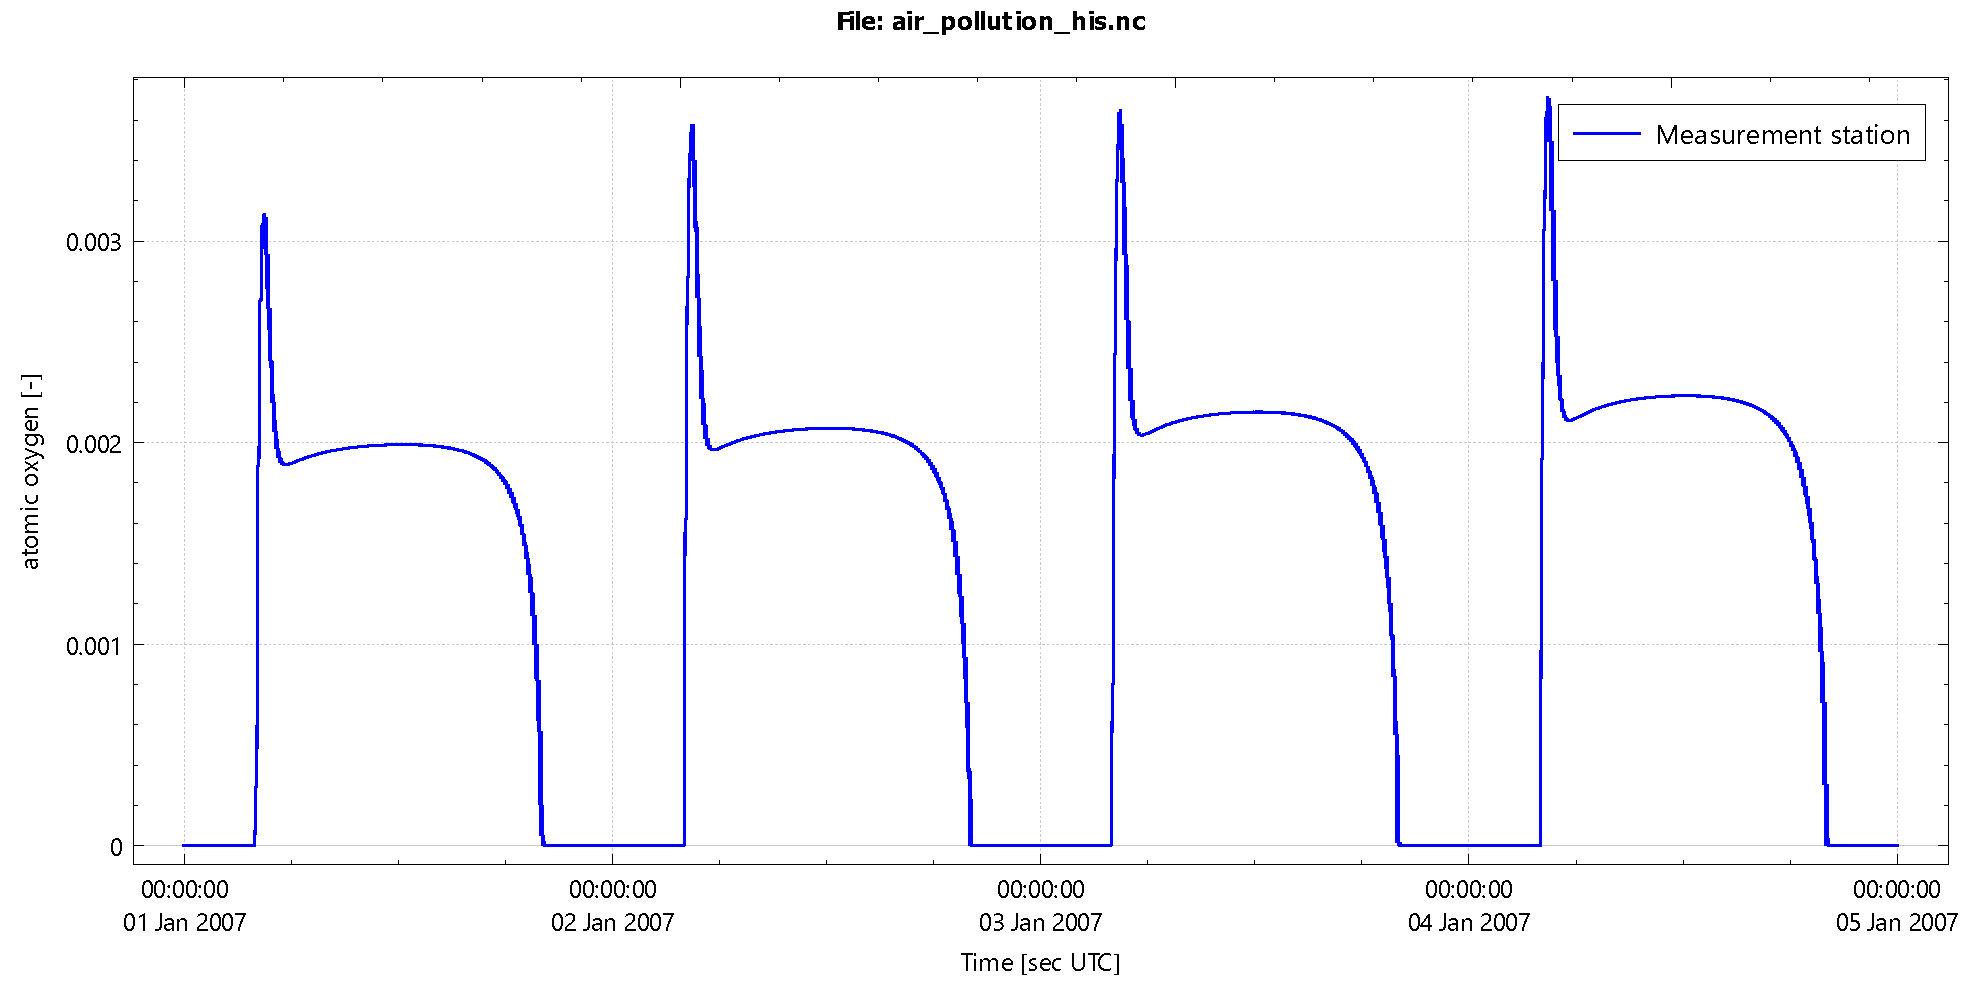
\includegraphics[width=\textwidth]{figures/atomic_oxygen_dt0d5.pdf}
        \caption{Concentration of Atomic Oxygen.}
    \end{subfigure}
    \begin{subfigure}{0.5\textwidth}
        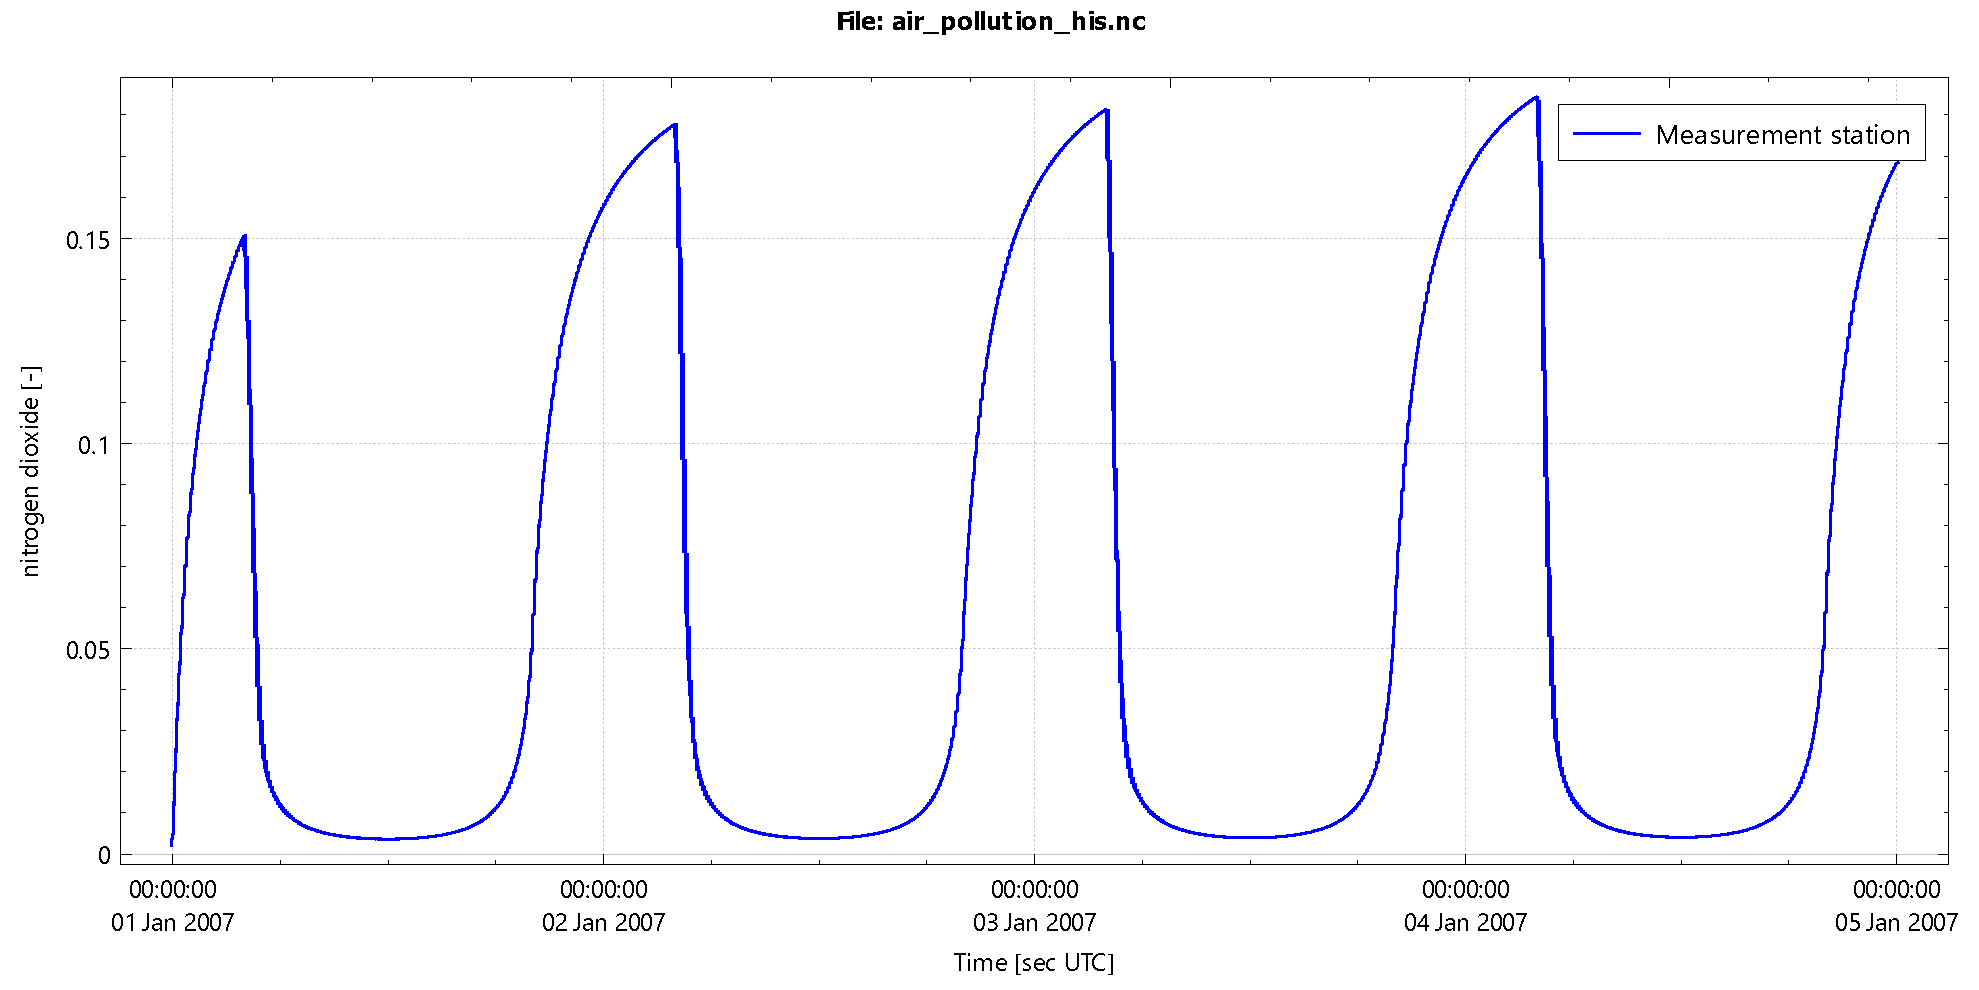
\includegraphics[width=\textwidth]{figures/nitrogen_dioxide_dt0d5.pdf}
        \caption{Concentration of Nitrogen Dioxide.}
    \end{subfigure}
    \begin{subfigure}{0.5\textwidth}
        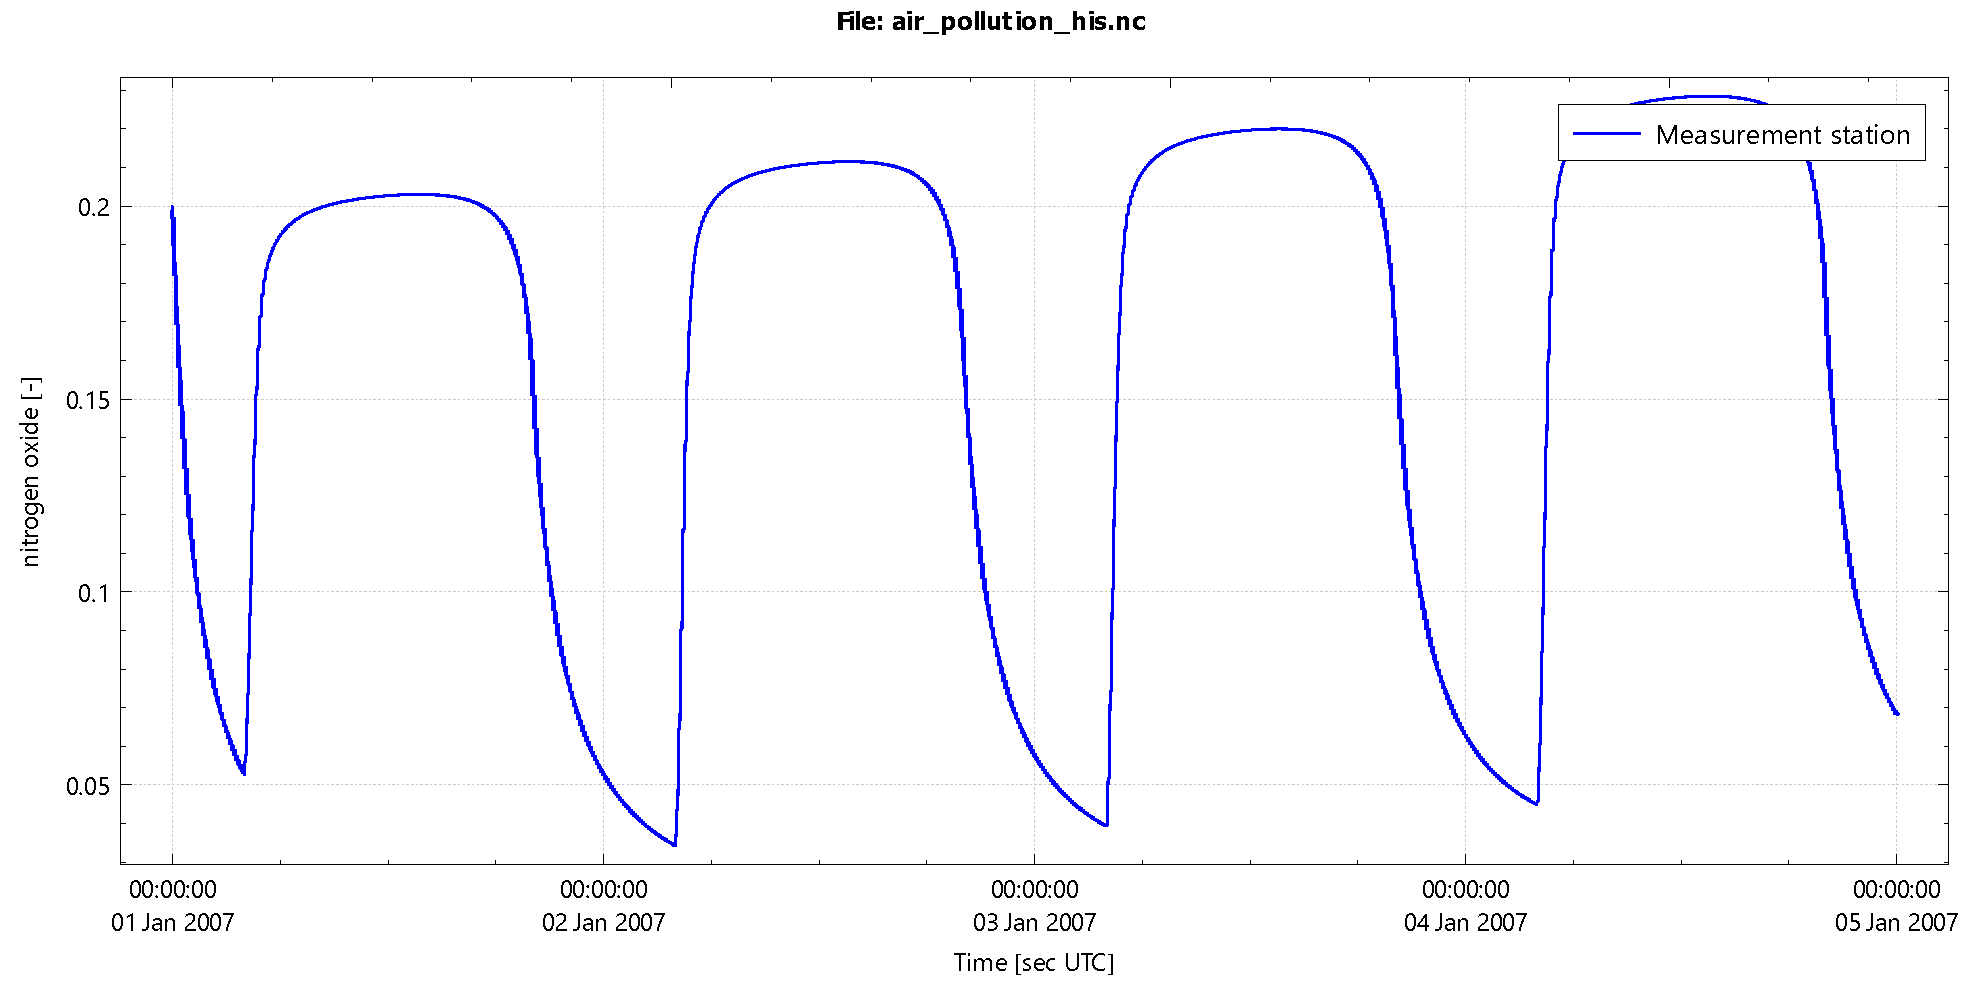
\includegraphics[width=\textwidth]{figures/nitrogen_oxide_dt0d5.pdf}
        \caption{Concentration of Nitrogen Oxide.}
    \end{subfigure}
    \begin{subfigure}{0.5\textwidth}
        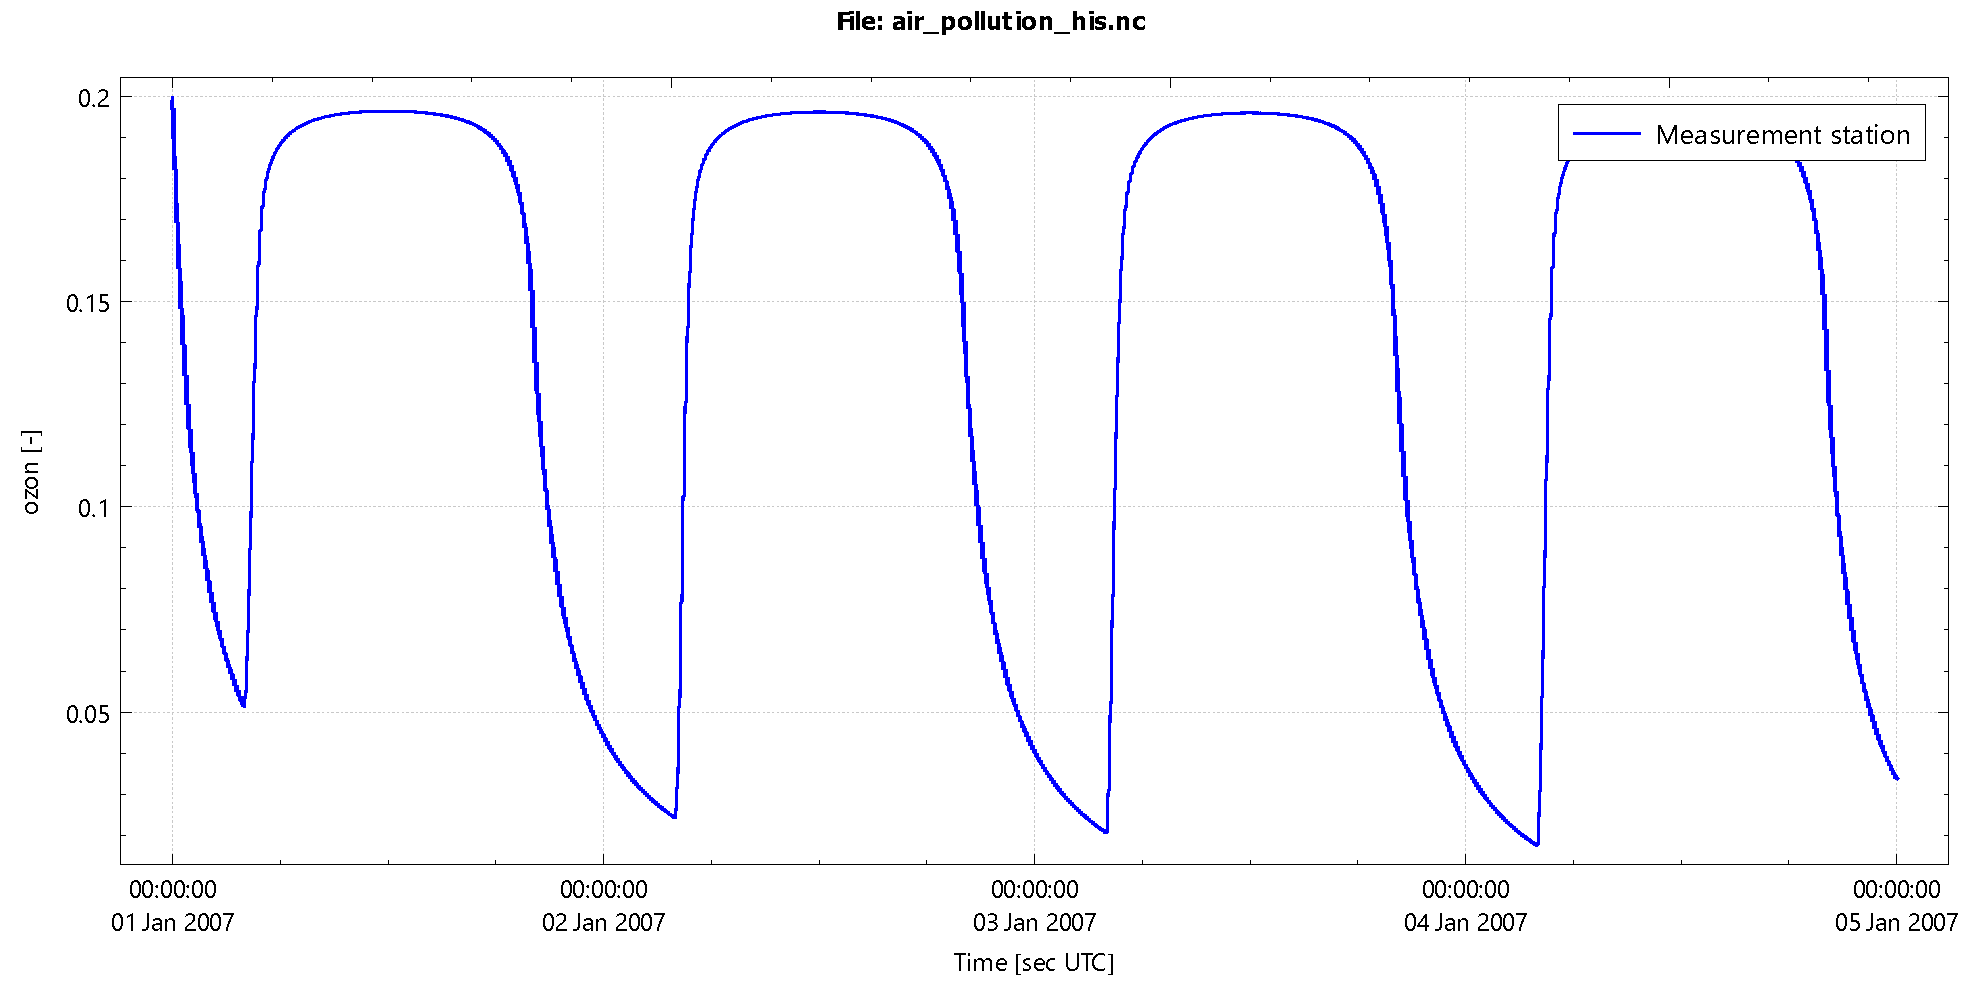
\includegraphics[width=\textwidth]{figures/ozon_dt0d5.pdf}
        \caption{Concentration of Ozon.}
    \end{subfigure}
    \caption[Air pollution experiment: $O$, $N_2$, $NO$ and $O_3$]{Result plots of the different constituents, compute with the fully implicit time integration method with a time step of \bqty{0.5}{\second}.}
\end{figure}

%------------------------------------------------------------------------------
\paragraph*{Different time integrators}
Numerical stability for different values of $\Dt$ are studied for Euler-explicit, Runga-Kutta-4 and the fully implicit $\Delta$-formulation.
%
\begin{longtable}{|>{\bfseries}p{6mm-12pt}|p{\textwidth/4-2mm-12pt}|p{\textwidth/4-2mm-12pt}|p{\textwidth/4-2mm-12pt}|p{\textwidth/4-2mm-12pt}|}
    \caption{Stability for different time integrators} \\%
    \rowcolor{mgreen1}
    & \textcolor{white}{\textbf{Time step\newline \bunit{\second}}}
    & \textcolor{white}{\textbf{Euler explicit}}
    & \textcolor{white}{\textbf{Runge-Kutta 4}}
    & \textcolor{white}{\textbf{Fully Implicit\newline \deltaformulation}}
    \\
    \topline
    \endfirsthead
    \rowcolor{mgreen1}
    & \textcolor{white}{\textbf{Time step\newline \bunit{\second}}}
    & \textcolor{white}{\textbf{Euler Explicit}}
    & \textcolor{white}{\textbf{Runge-Kutta 4}}
    & \textcolor{white}{\textbf{Fully Implicit\newline \deltaformulation}}
    \\
    \midline
    \endhead
    \endfoot
    \bottomline
    \endlastfoot
    1 & 0.5 & -  & \checkmark & \checkmark  \\
    \midline
    2 & 60 & \checkmark  & \checkmark  &  \checkmark \\
    \midline
    3 & 120 & Unstable & \checkmark &  \checkmark \\
    \midline
    4 & 180 & - & Unstable & \checkmark \\
    \midline
    5 & 240 & - & - & \checkmark \\
    \midline
    6 & 300 & - & - & \checkmark \\
    \midline
    7 & 900 & - & - & \checkmark \\
    \midline
    8 & 1800 & - & - & \checkmark \\
    \midline
    9 & 3600 & - & - & \checkmark \\
\end{longtable}

%
%------------------------------------------------------------------------------
\subsection{Brusselator}\label{sec:num_exp_brusselator}
%--------------------------------------------------------------------------------
Some numerical results of the Brusselator example (\autoref{sec:brusselator}) is:
\begin{figure}[H]
    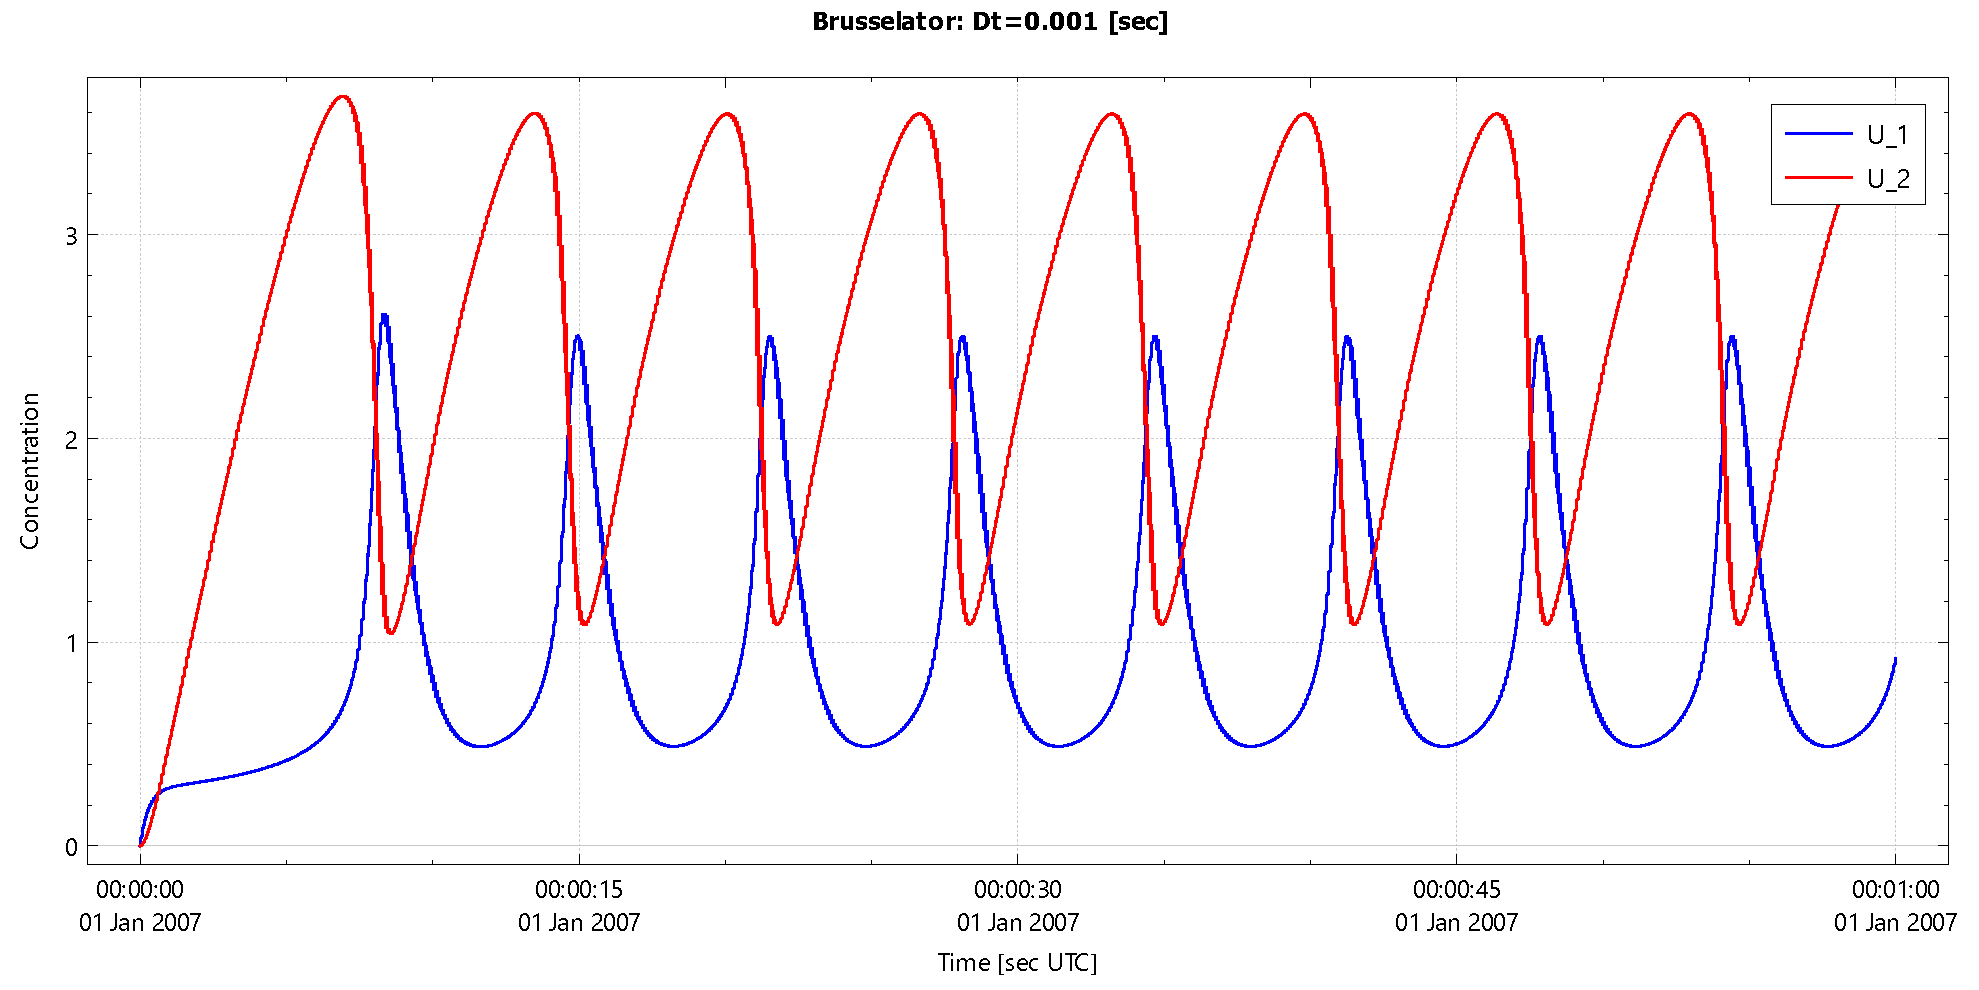
\includegraphics[width=\textwidth]{figures/brusselator_imp_dt=0d001.pdf}
    \caption[Brusselator experiment: $\Dt = 0.001\ \bunit{\second}$]{Fully Implicit: $\Dt=0.001$\ \bunit{\second}, $k_1=1$, $k_2=2.5$. }\label{fig:brusselator_reference}
\end{figure}
The solution presented in \autoref{fig:brusselator_reference} is assumed to be the reference (analytic) solution of \autoref{eq:brusselator}.
%
\begin{figure}[H]
    \begin{subfigure}{0.5\textwidth}
        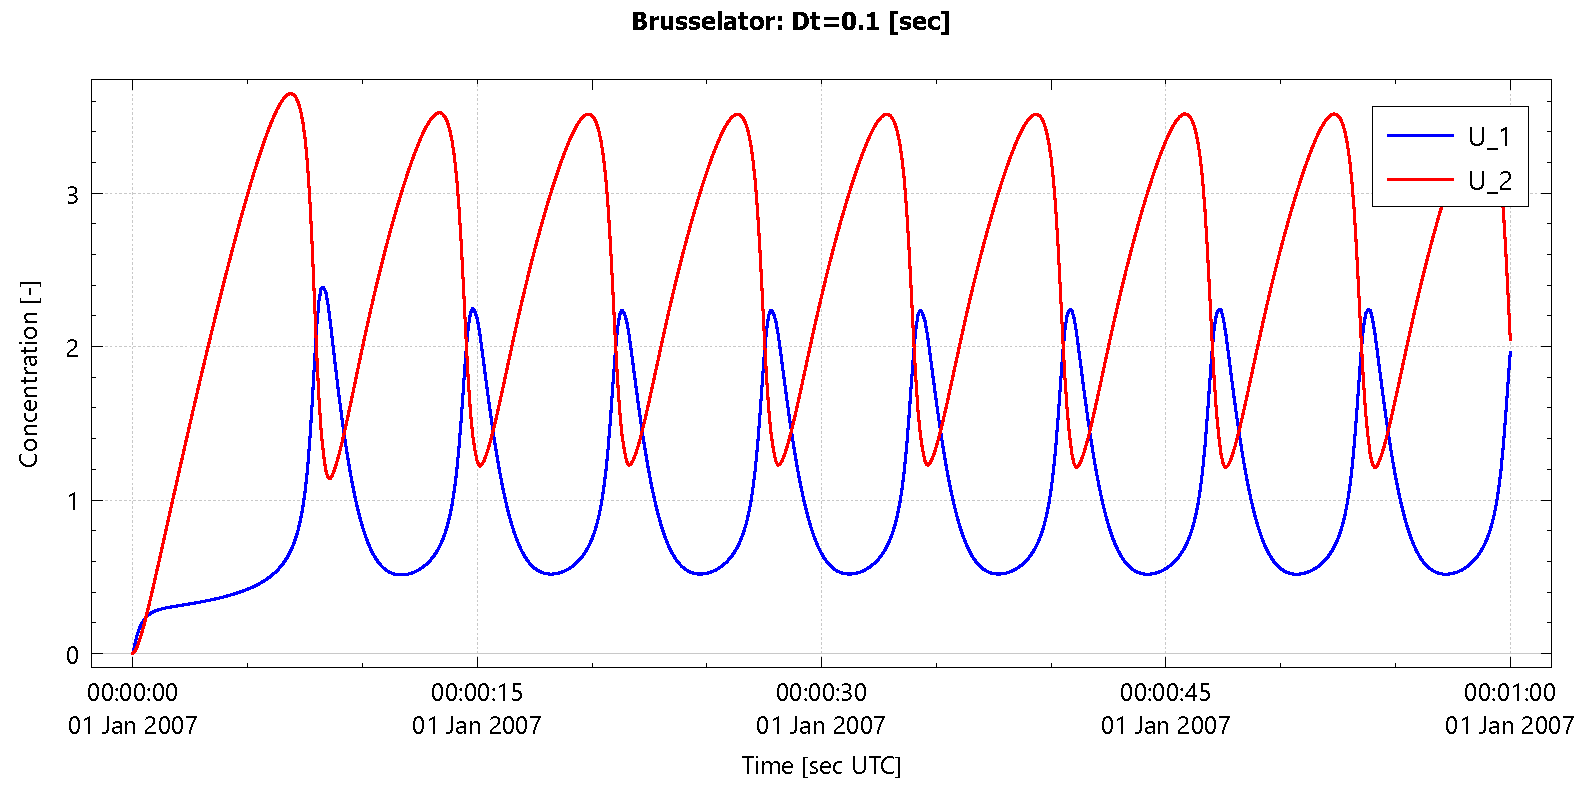
\includegraphics[width=\textwidth]{figures/brusselator_imp_dt=0d10.pdf}
        \caption{Fully Implicit: $\Dt=\bqty{0.1}{\second}$, $k_1=1$, $k_2=2.5$}
    \end{subfigure}
    \begin{subfigure}{0.5\textwidth}
        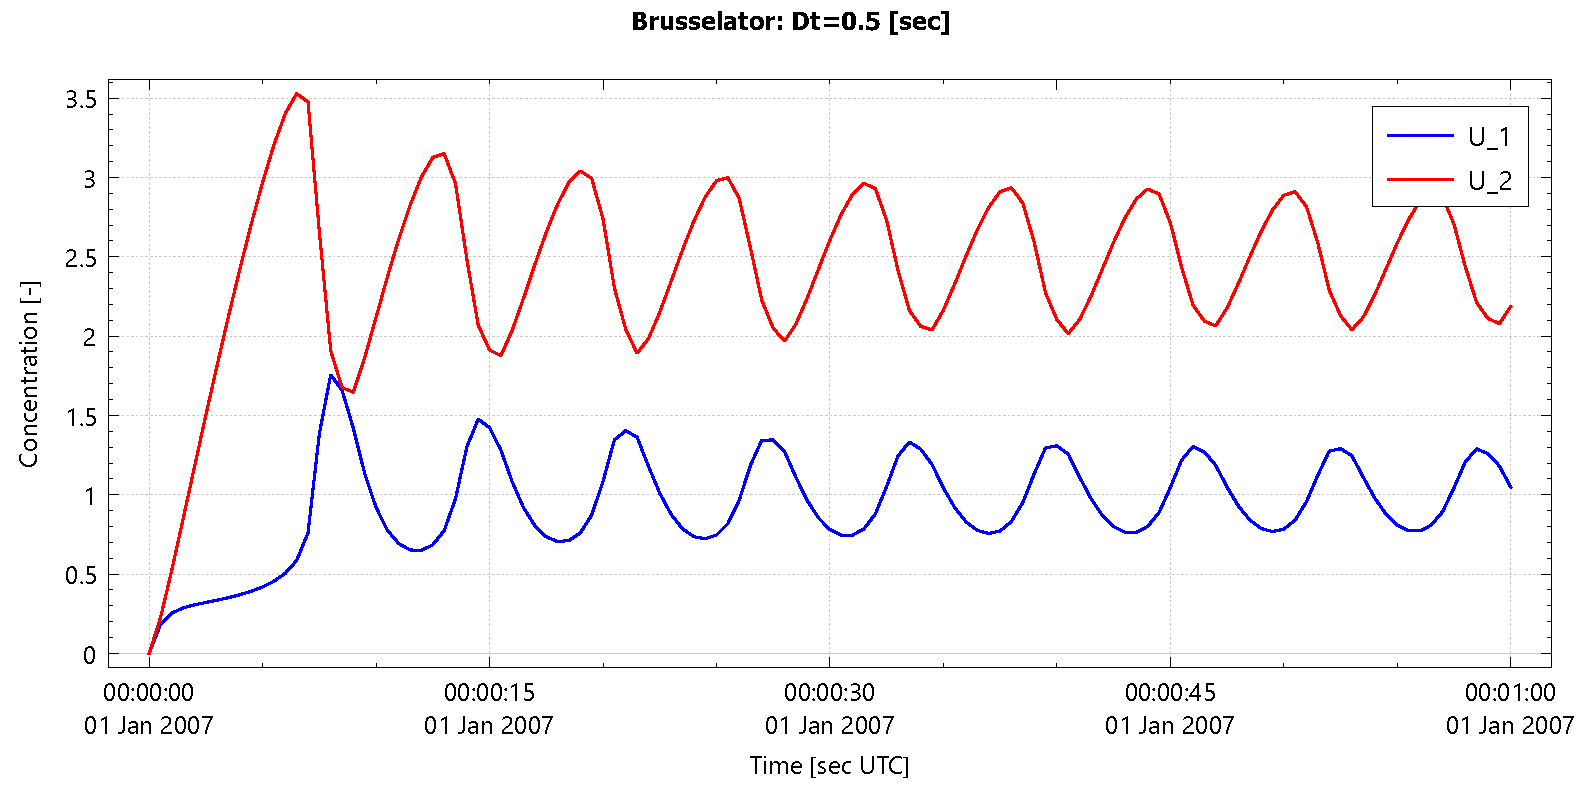
\includegraphics[width=\textwidth]{figures/brusselator_imp_dt=0d50.pdf}
        \caption{Fully Implicit: $\Dt=\bqty{0.5}{\second}$, $k_1=1$, $k_2=2.5$}
    \end{subfigure}
    \caption[Brusselator experiment: $\Dt = 0.1, 0.5\ \bunit{\second}$]{Result plots for constant value of $k_1 = 1$ and $k_2 =2.5$, computed with a fully implicit ($\Delta$ formulation) time integration method for different time steps $\Dt = 0.1, 0.5\ \bunit{\second}$.}
\end{figure}
Extra attention is needed for the Fully Implicit time integration with larger time step:
\begin{figure}[H]
    \begin{subfigure}{0.5\textwidth}
        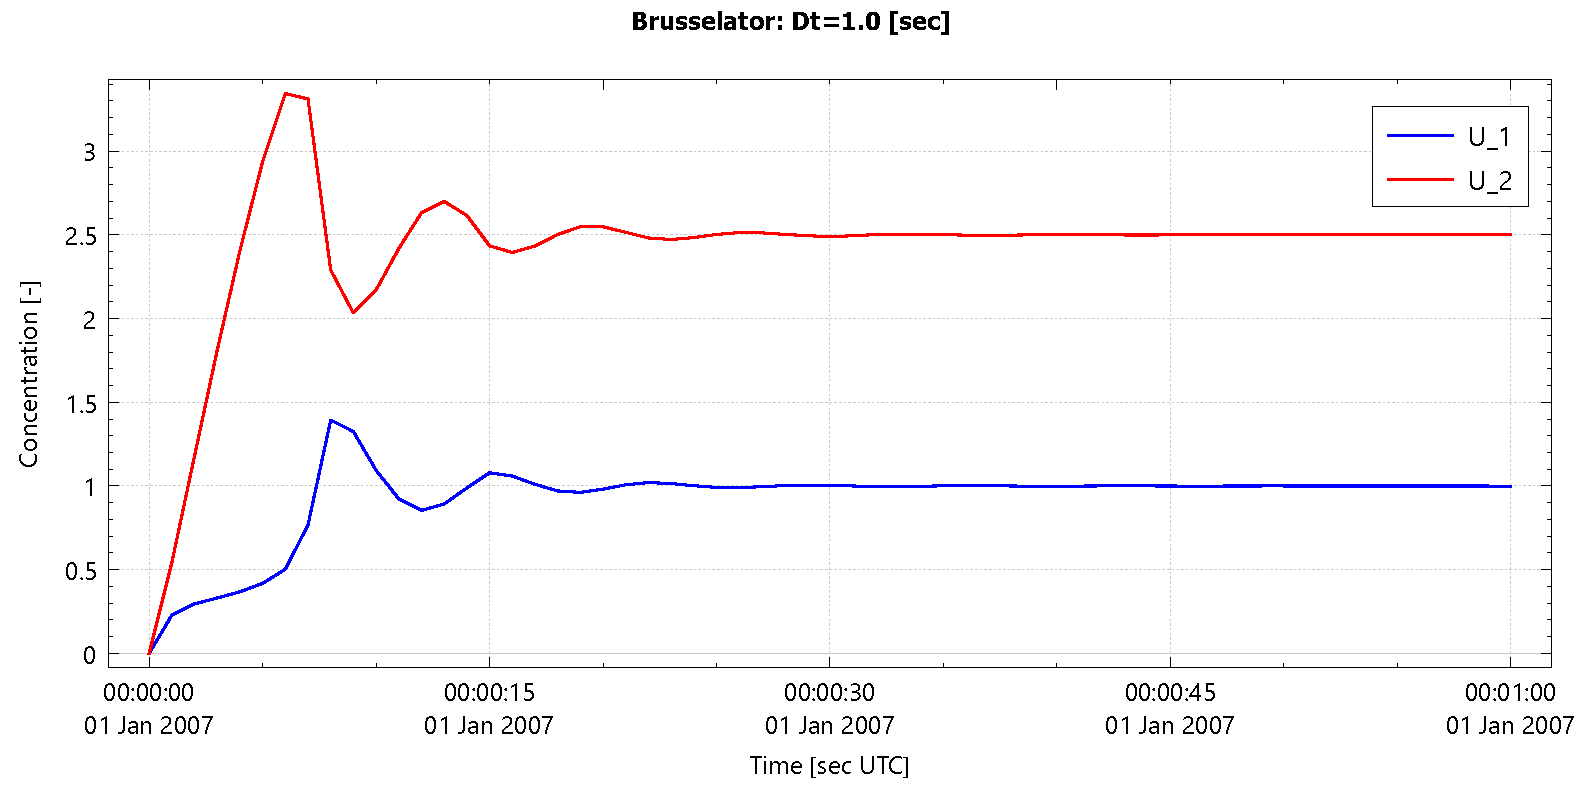
\includegraphics[width=\textwidth]{figures/brusselator_imp_dt=1d00.pdf}
        \caption{Fully Implicit: $\Dt=\bqty{1.0}{\second}$, $k_1=1$, $k_2=2.5$}\label{fig:imp_dt=1d00}
    \end{subfigure}
    \begin{subfigure}{0.5\textwidth}
        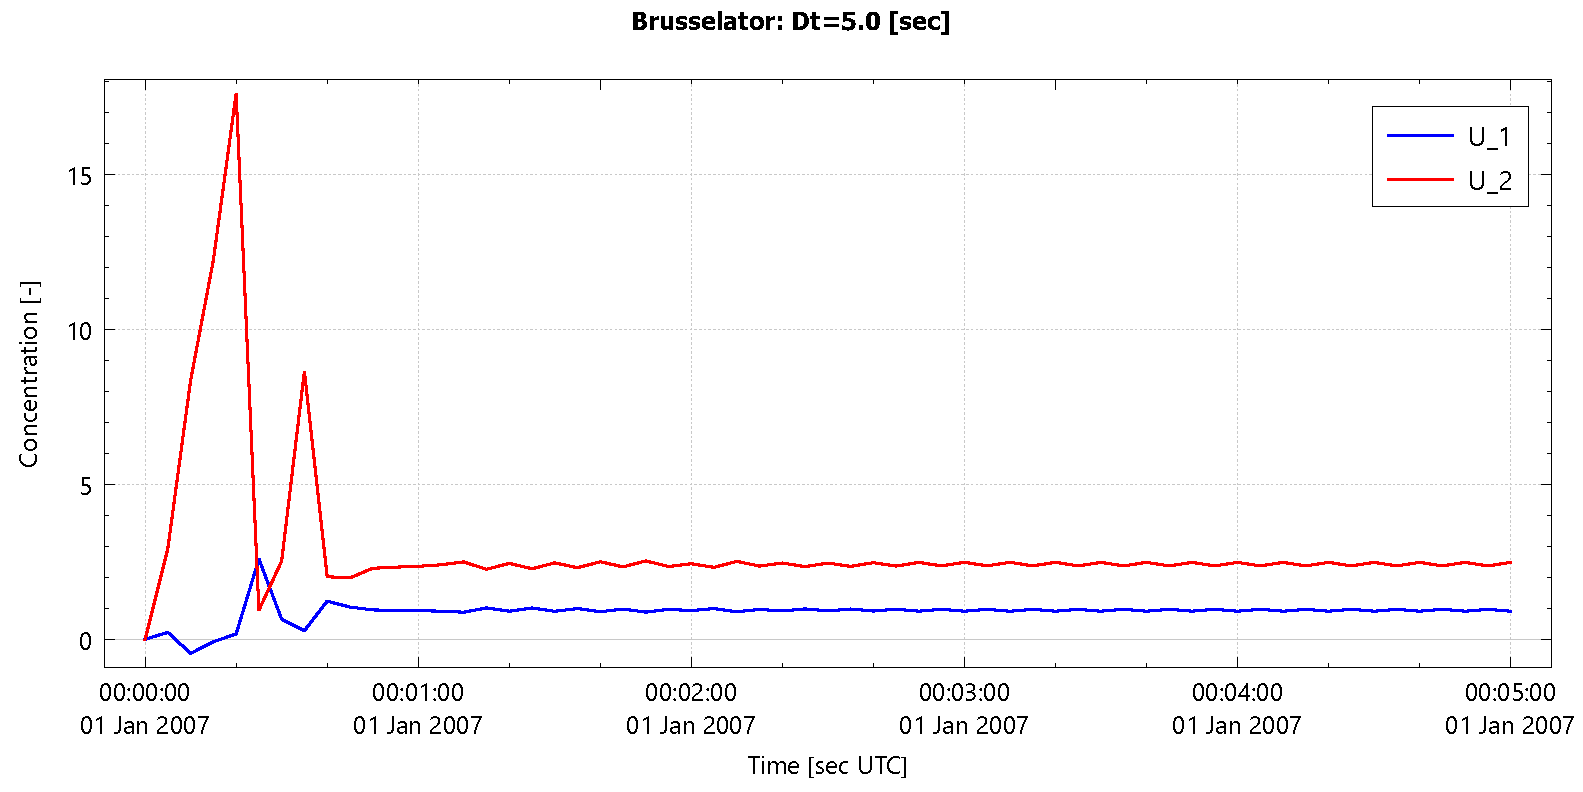
\includegraphics[width=\textwidth]{figures/brusselator_imp_dt=5d00.pdf}
        \caption{Fully Implicit: $\Dt=\bqty{5.0}{\second}$, $k_1=1$, $k_2=2.5$}\label{fig:imp_dt=5d00}
    \end{subfigure}
    \caption[Brusselator experiment: $\Dt = 1.0, 5.0\ \bunit{\second}$]{Result plots for constant value of $k_1 = 1$ and $k_2 =2.5$, computed with a fully implicit ($\Delta$ formulation) time integration method for different time steps $\Dt = 1.0, 5.0\ \bunit{\second}$.
    }
\end{figure}
\Autoref{fig:imp_dt=1d00} converge to the equilibrium state $(u_1, u_2) = (1.0, 2.5)$ and
\Autoref{fig:imp_dt=5d00} looks to converge to the equilibrium state $(u_1, u_2) = (1.0, 2.5)$ but is still wiggling after \bqty{5}{\minute} of simulation time (even after one day --- not presented here).
How these equations are discretized is given in \autoref{sec:brusselator_discretization}.

%------------------------------------------------------------------------------
\paragraph*{Different time integrators}
Numerical stability for different values of $\Dt$ are studied for the Runga-Kutta-4 and fully implicit \deltaformulation.
%
\begin{longtable}{|>{\bfseries}p{6mm-12pt}|p{\textwidth/3-2mm-12pt}|p{\textwidth/3-2mm-12pt}|p{\textwidth/3-2mm-12pt}|}
    \caption{Stability of different time integrators for the Brusselator.} \\%
    \rowcolor{mgreen1}
    & \textcolor{white}{\textbf{Time step\newline \bunit{\second}}}
    & \textcolor{white}{\textbf{Runge-Kutta 4}}
    & \textcolor{white}{\textbf{Fully Implicit\newline \deltaformulation}}
    \\
    \topline
    \endfirsthead
    \rowcolor{mgreen1}
    & \textcolor{white}{\textbf{Time step\newline \bunit{\second}}}
    & \textcolor{white}{\textbf{Runge-Kutta 4}}
    & \textcolor{white}{\textbf{Fully Implicit\newline \deltaformulation}}
    \\
    \midline
    \endhead
    \endfoot
    \bottomline
    \endlastfoot
    1 & 0.1 & \checkmark & \checkmark  \\
    \midline
    2 & 0.2  & \checkmark &  \checkmark   \\
    \midline
    3 & 0.5 & \checkmark &  \checkmark   \\
    \midline
    4 & 1.0 & Unstable &   \checkmark  \\
    \midline
    5 & 2.0 &   &   \checkmark  \\
    \midline
    6 & 5.0 &   &   \checkmark  \\
    \midline
\end{longtable}
